
\subsubsection{Dual Contouring}

\begin{frame}
	\frametitle{From Voxel to Mesh Geometry}
	\vspace{-0.8cm}
	\begin{center}
	\textbf{Goal:} Extract isosurface from voxel information	
	\end{center}
\vspace{-0.5cm}	
\begin{minipage}[t]{0.4\linewidth}
		\begin{block}{Marching Cubes}
	\begin{enumerate}
		\item<2-> Identify boundary voxels
		\item<3-> Locate sign changes on cube edges
		\item<4-> Reconstruct surface
	\end{enumerate}
	
	\end{block}
	\only<1>{
\begin{figure}	
		\centering
	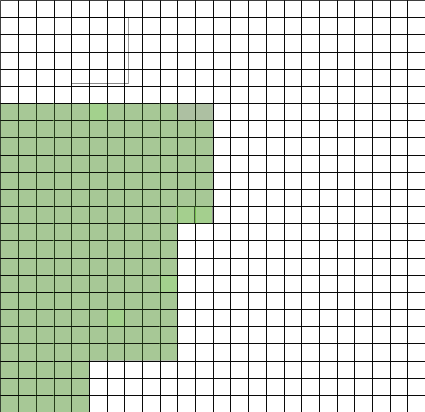
\includegraphics[width=.6\textwidth]{Pictures/DC/MC1.png} %\caption{Marching Cubes}
\end{figure} }
	\only<2>{
		\begin{figure}	
			\centering
			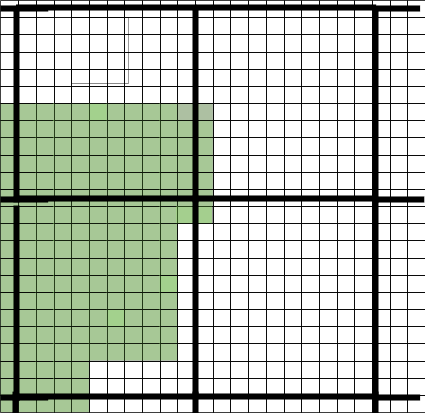
\includegraphics[width=.6\textwidth]{Pictures/DC/MC2.png} %\caption{Marching Cubes}
			\end{figure}}
		\only<3>{
			\begin{figure}	
			\centering
			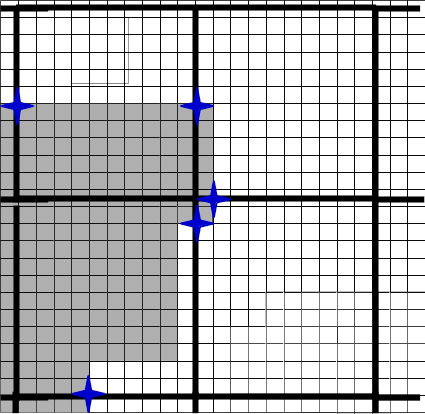
\includegraphics[width=.6\textwidth]{Pictures/DC/MC3.png} %\caption{Marching Cubes}
			\end{figure}}
				\only<4->{
					\begin{figure}	
					\centering
					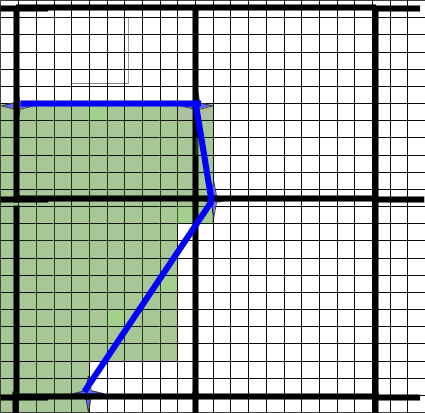
\includegraphics[width=.6\textwidth]{Pictures/DC/MC4.png} %\caption{Marching Cubes}
					\end{figure}}
				

\end{minipage}%
\hfill%
\begin{minipage}[t]{0.4\linewidth}
\begin{block}<5->{Dual Contouring}
	\begin{enumerate}
		\item<6-> Identify boundary voxels
		\item<7-> Locate position inside boundary voxel
		\item<8-> Reconstruct surface
	\end{enumerate}
	
\end{block}
	\only<5>{
\begin{figure}	
	\centering
	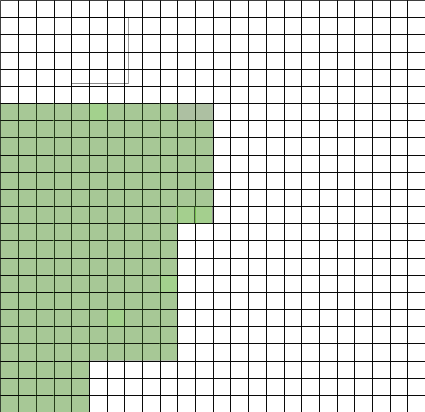
\includegraphics[width=.6\textwidth]{Pictures/DC/MC1.png} %\caption{Dual Contouring}
\end{figure} }
	\only<6>{
		\begin{figure}	
		\centering
		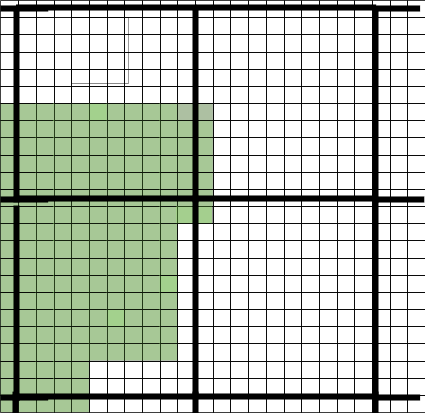
\includegraphics[width=.6\textwidth]{Pictures/DC/MC2.png} %\caption{Dual Contouring}
		\end{figure}}
	\only<7>{
		\begin{figure}	
		\centering
		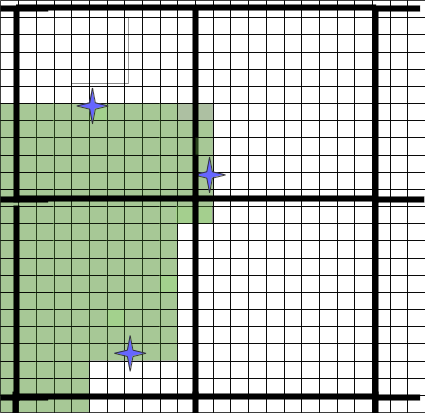
\includegraphics[width=.6\textwidth]{Pictures/DC/DC3.png} %\caption{Dual Contouring}
		\end{figure}}
			\only<8->{
				\begin{figure}	
				\centering
				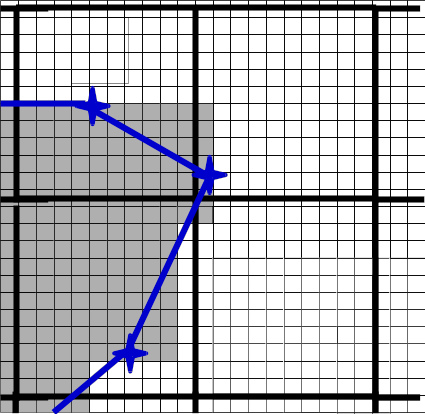
\includegraphics[width=.6\textwidth]{Pictures/DC/DC4.png} %\caption{Dual Contouring}
	\end{figure}}
	
\end{minipage}
\only<9>{
\begin{minipage}[t]{0.4\linewidth}
{$\rightarrow Triangles$}
\end{minipage}
\hfill
\begin{minipage}[t]{0.4\linewidth}
{$\rightarrow Quads$}
\end{minipage}}
\end{frame}


\begin{frame}
	\frametitle{Dual Contouring}
	\begin{overlayarea}{\textwidth}{.25 \textheight}
	Dual contouring on two different scales:
	\frametitle{Two-grid Dual Contouring}
	\begin{overlayarea}{\textwidth}{0.9 \textheight}
	\begin{minipage}{0.45\textwidth}
	\begin{block}{\centering Coarse grid}
	\vspace{-0.5cm}
	\begin{figure}
	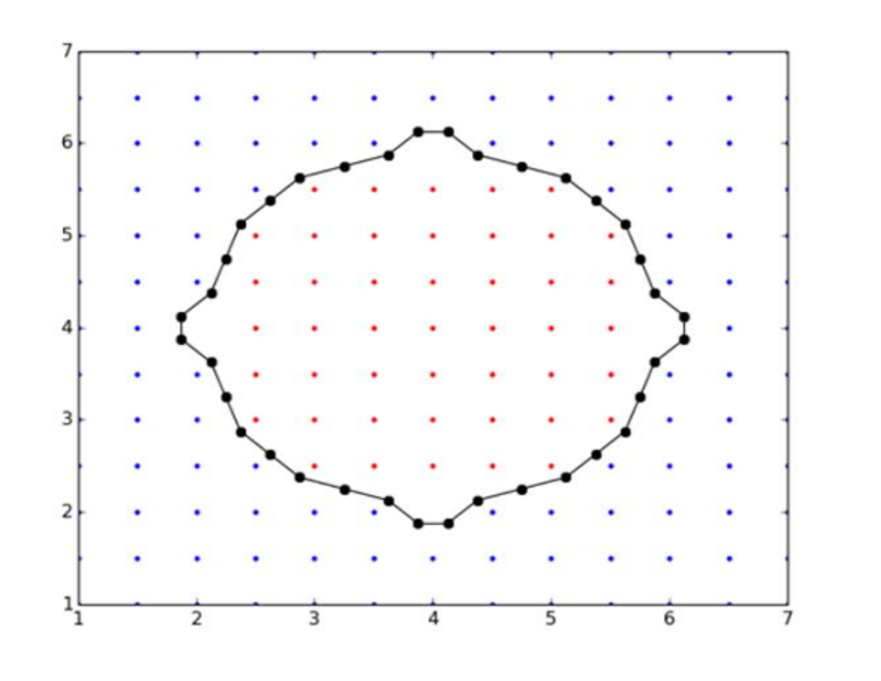
\includegraphics[scale=0.35]{Pictures/DC/DC_1_Coarse.pdf}
	\end{figure}
	\begin{itemize}
	\item Coarse quads used in \textcolor{red}{parametrization}
	\end{itemize}
	\end{block}
	\end{minipage}
	\hfill%
	\begin{minipage}{0.45\textwidth}
	\begin{block}{\centering Fine grid}
	\vspace{-0.5cm}
	\begin{figure}
	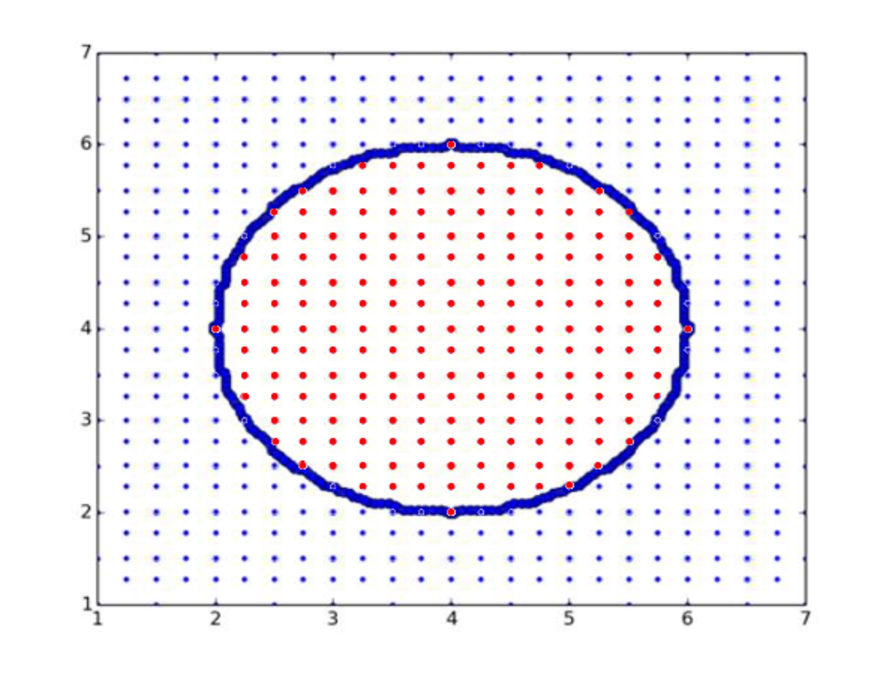
\includegraphics[scale=0.35]{Pictures/DC/DC_1_Fine.pdf}
	\end{figure}
	\begin{itemize}
	\item Fine vertices used for \textcolor{red}{projection}
	\end{itemize}
	\end{block}
	\end{minipage}
	\end{overlayarea}
\end{frame}

%\subsection{B--Spline}

\subsection{Projection and Parametrization}
\begin{frame}{Projection and Parametrization}
%\framesubtitle{Least square fitting}
\begin{overlayarea}{\textwidth}{.9 \textheight}
%\begin{minipage}{0.45\textwidth}
\begin{enumerate}
\visible<1->{\item Use coarse quad from Dual Contouring}
\visible<2->{\item Project grid points from fine grid onto plane}
\visible<3->{\item Find corresponding parameters for B-Spline surface $\left[u,v\right] \in \left[0,1\right]^2$}
\visible<4->{\alert<4->{\item[$\Rightarrow$] Peter's scheme}}
\end{enumerate}
%\end{overlayarea}
%\begin{overlayarea}{\textwidth}{.85 \textheight}
%\end{minipage}
\vspace{-0.5cm}
%\begin{columns}
%\column{.35\textwidth}
%\begin{overlayarea}{\textwidth}{\textheight}
\begin{figure}
\visible<1->{
\tdplotsetmaincoords{60}{110}
\begin{tikzpicture}[scale = 1.5,tdplot_main_coords]
\coordinate (O) at (-1,-1,0);
\coordinate[dot] (A) at (0,0,0);
\coordinate[dot] (B) at (1,0,0);
\coordinate[dot] (C) at (1.2,1.5,0);
\coordinate[dot] (D) at (0,1,0);
\visible<3->{
\coordinate[dot] (E) at (1.4,2.0,-0.5);
\coordinate[dot] (F) at (0,1.7,-0.8);
\draw[thick] (D) -- (F) -- (E) -- (C);}

\coordinate (P1) at (.5,.4,1);
\coordinate (P2) at (1,1,1);
\coordinate (P3) at (0.2,0.2,2);
\coordinate (P4) at (0.1,1.3,1);


\coordinate (Q1) at (.5,.4,0);
\coordinate (Q2) at (1,1,0);
\coordinate (Q3) at (0.2,0.2,0);
\coordinate (Q4) at (0.1,0.9,0);



\draw[thick,->] (O) -- ($(O)+(.5,0,0)$) node[anchor=north east]{$x$};
\draw[thick,->] (O) -- ($(O)+(0,.5,0)$) node[anchor=north west]{$y$};
\draw[thick,->] (O) -- ($(O)+(0,0,.5)$) node[anchor=south]{$z$};

\draw[thick] (A) -- (B) -- (C) -- (D) -- (A);

\visible<2-4>{
\draw (P1) node[thick,cross,red,label = {$P_1$}] {};
\draw[red,dashed] (P1) -- (Q1);
\draw (Q1) node[thick,cross,red] {};
\draw (P2) node[thick,cross,red,label = {$P_2$}] {};
\draw[red,dashed] (P2) -- (Q2);
\draw (Q2) node[thick,cross,red] {};
\draw (P3) node[thick,cross,red,label = {$P_3$}] {};
\draw[red,dashed] (P3) -- (Q3);
\draw (Q3) node[thick,cross,red] {};
}
\visible<3->{
\draw (P4) node[thick,cross,red,label = {$P_4$}] {};
\draw[red,dashed] (P4) -- (Q4);
\draw (Q4) node[thick,cross,red] {};

}
\draw (A) node[label = left:{$A$}]{};
\draw (B) node[label = left:{$B$}]{};
\draw (C) node[label = right:{$C$}]{};
\draw (D) node[label = right:{$D$}]{};
\visible<3->{
\draw (E) node[label = right:{$E$}]{};
\draw (F) node[label = right:{$F$}]{};}
\visible<3->{
\coordinate[dot] (A2) at (0,0,1);
\coordinate[dot] (B2) at (1,0,1);
\coordinate[dot] (D2) at (0.,1.5,0.9);
\coordinate[dot] (C2) at (1,1.9,1);
\draw [dashed] (A2)--(D2) --(C2) -- (B2) -- (A2);
%\draw (C2) node[label = right:{$C'$}]{};
%\draw (D2) node[label = right:{$D'$}]{};
%\draw (A2) node[label = right:{$A'$}]{};
%\draw (B2) node[label = right:{$B'$}]{};
}
\end{tikzpicture}
}
\end{figure}
%\end{overlayarea}

%\column{.5\textwidth}
%\begin{overlayarea}{\textwidth}{\textheight}
%\only<3->{
%\begin{block}{Problem:}
%\begin{itemize}
%\item Fit B-Spline surface, that is C0 and C1 continuous on the borders
%\end{itemize}
%\end{block}
%
%\begin{block}{Solution:}
%\begin{enumerate}
%\item Method: Peter's scheme
%\item Solve (coupled) global system of equations
%\end{enumerate}
%\end{block}
%
%}
%\end{overlayarea}
%\end{columns}
\end{overlayarea}
\end{frame}

%\begin{frame}
%
%	\frametitle{Projection and Parametrization}
%	
%	\begin{itemize}
%	\item Points from finer grid are projected to quads of the coarser grid 
%	\item Parameters \textit{u} and \textit{v} are found for each quad
%	\item This information is needed for the algorithms in the last part of the pipeline
%	\end{itemize}
%	\begin{figure}
%	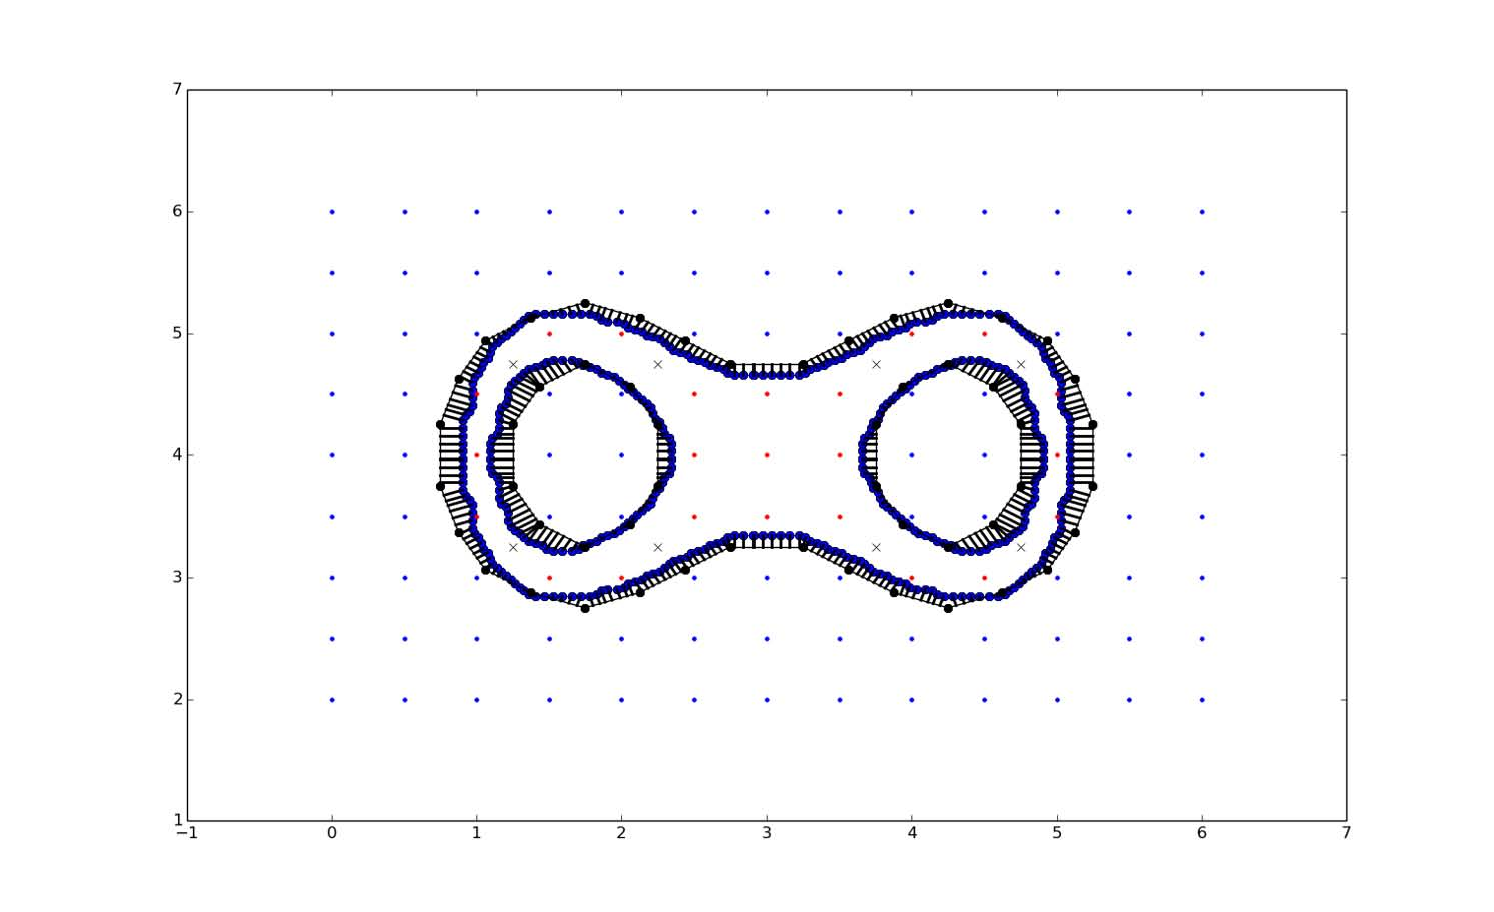
\includegraphics[scale=0.35]{Pictures/DC/DC_2.pdf}
%	\end{figure}
%	
%\end{frame}





